\documentclass[a4paper,12pt]{article}
\usepackage{graphicx}
\usepackage{bm,amssymb}
\usepackage{mathrsfs}
\usepackage[unicode,colorlinks=true,filecolor=blue, menucolor=black, linkcolor=black, citecolor=black,pagebackref=white]{hyperref}
\usepackage[utf8]{inputenc}
\usepackage[russian]{babel}
\usepackage{amsmath}
\usepackage{feynmp}
\usepackage{caption}
\usepackage{cite}
\usepackage[left=2cm,right=2cm, top=2cm,bottom=2cm,bindingoffset=0cm]{geometry}
\begin{document}
\title{Семинар по теме: <<Вариационные задачи>>}
\maketitle
\subsection*{Общая теория}

Вариационные задачи, возникающие чаще всего в приложениях, сводятся
к минимизации функционала (в механике он называется ``действием''):
\[
S\left[x\left(t\right)\right]=\int_{t_{1}}^{t_{2}}L(x(t),\dot{x}(t),t)dt
\]

\noindent
с некой функцией $L(x,\dot{x},t)$, называемой в механике ``функцией
Лагранжа'' или ``лагранжианом''. - некая функция трех переменных
(ее мы назовём ``лагранжианом''). Этот функционал ставит в соответствие
функции $x(t)$ некое число. Вариационная задача заключается в нахождении
такой функции $x(t)$, чтобы действие на ней было минимальным (или
максимальным).
\noindent
Для обычных функций $f(x)$ условие экстремума можно записать следующим
образом. Точка $x=x_{min}$ является экстремумом, если разложение
до линейного порядка по $\delta x=x-x_{min}$ около этой точки зануляется:

\[
f(x)-f(x_{min})=f^{\prime}(x_{min})\delta x+\underline{O}(\delta x^{2})=0\Rightarrow f^{\prime}(x_{min})=0
\]

\noindent
Это можно обобщить и на случай функционала. Пусть $x_{min}(t)$ -
функция, на которой достигается экстремум функционала $S[x(t)]$.
Тогда необходимо слабо возмутить эту функцию, рассмотрев значение
функционала на функции $x(t)=x_{min}(t)+\delta x(t)$ и найти линейную
по $\delta x$ часть приращения функционала:
\begin{multline*}
\delta S=S[x_{min}(t)+\delta x(t)]-S[x_{min}(t)]\equiv\\
\equiv \int_{t_{1}}^{t_{2}}\left(L(x_{min}(t)+\delta x(t),\dot{x}_{min}(t)+\dot{\delta x}(t),t)-L(x_{min}(t),\dot{x}_{min}(t),t)\right)dt=\\
=\int_{t_{1}}^{t_{2}}\left(\frac{\partial L}{\partial x}\cdot\delta x(t)+\frac{\partial L}{\partial\dot{x}}\dot{\delta x}(t)\right)dt+\underline{O}(\delta x^{2})
\end{multline*}

\noindent
Второе слагаемое можно проинтегрировать по частям. Для того, чтобы
не рассматривать внеинтегральный член, добавим к нашей вариационной
задаче так называемое условие закреплённых концов, а именно: функционал
минимизируется на таких функциях $x(t)$, что $x(t_{1})\equiv x_{1}$
и $x(t_{2})\equiv x_{2}$ (значения на краях фиксированы). Это значит,
что вариация удовлетворяет $\delta x(t_{1})=\delta x(t_{2})=0$, поэтому
внеинтегрального члена не будет:
\[
\delta S=\int_{t_{1}}^{t_{2}}\left(\frac{\partial L}{\partial x}-\frac{d}{dt}\frac{\partial L}{\partial\dot{x}}\right)\delta x(t)dt
\]

\noindent
Требование $f^{\prime}(x_{min})=0$ в нашем случае заменяется на требование
равенства нулю так называемой вариационной производной:
\[
\frac{\delta S}{\delta x}\underset{def}{\equiv}\frac{\partial L}{\partial x}-\frac{d}{dt}\frac{\partial L}{\partial\dot{x}}=0
\]

\noindent
Это - обыкновенное дифференциальное уравнение; и функция, на которой
действие достигает экстремального значения, обязана ему удовлетворять.
Это уравнение называется уравнением Эйлера-Лагранжа.


\subsection*{Примеры вариационных задач}


\subsubsection*{Геометрическая оптика}

Первый пример, в которых возникают вариационные задачи - это принцип
Ферма в геометрической оптике, гласящий, что свет распространяется
по такой траектории, на которой время его движения минимально. Запишем
это на условие языке вариационной задачи. Пусть показатель преломления
как-то меняется в пространстве $n(\mathbf{r})$; в этом случае, скорость
света в среде записывается как $v(\mathbf{r})=\frac{c}{n(\mathbf{r})}$.
Пусть луч света описывает некую траекторию $\left\{ \mathbf{r}(t),t\in(t_{1},t_{2})\right\} $
(при этом параметр $t$ попросту параметризует эту траекторию; не
стоит его путать со временем). Время распространения на этой траектории
тогда записывается в виде криволинейного интеграла:
\[
T[\mathbf{r}(t)]=\oint_{\mathbf{r}(t)}\frac{dr}{v(\mathbf{r})}\equiv\frac{1}{c}\int_{t_{1}}^{t_{2}}n(\mathbf{r}(t))\left|\dot{\mathbf{r}}(t)\right|dt
\]

\noindent
В трехмерном пространстве ``лагранжиан'' этого функционала зписывается
как (опуская несущественный фактор $1/c$):

\[
L(x,y,z,\dot{x},\dot{y},\dot{z})\equiv n(\mathbf{r})|\dot{\mathbf{r}}|=n(x,y,z)\sqrt{\dot{x}^{2}+\dot{y}^{2}+\dot{z}^{2}}
\]

\noindent
В случае многих координат необходимо писать систему уравнений Эйлера-Лагранжа
на каждую из координат, то есть:

\[
\begin{cases}
\frac{\partial L}{\partial x} & =\frac{d}{dt}\frac{\partial L}{\partial\dot{x}}\\
\frac{\partial L}{\partial y} & =\frac{d}{dt}\frac{\partial L}{\partial\dot{y}}\\
\frac{\partial L}{\partial z} & =\frac{d}{dt}\frac{\partial L}{\partial\dot{z}}
\end{cases}
\]



\subsubsection*{Классическая механика}

Уравнения классической механики также можно переформулировать на вариационном
языке. В общем случае оказывается, что лагранжиан записывается как
$L=T-\Pi$, где $T$ - кинетическая энергия, а $\Pi$ - потенциальная.
В частности, для классической частицы массы $m$, движущейся в одномерье
в потенциале $U(x)$, лагранжиан имеет вид 
\[
L(x,\dot{x})=\frac{m\dot{x}^{2}}{2}-U(x)
\]

\noindent
и соответствующее уравнение Эйлера-Лагранжа имеет вид просто второго
закона Ньютона:
\[
m\ddot{x}=-\frac{\partial U}{\partial x}
\]



\subsection*{Задача 1}

Пусть теперь свет распространяется в среде с переменным показателем
преломления, с зависимостью:
\[
n\left(x,y\right)=n_{0}-\beta xy
\]

\noindent
причём параметр $\beta$ мал. Исследуем траекторию, по которой луч
будет двигаться из точки $(0;0)$ в точку $(L;0)$.


\subsubsection*{Решение}

Пусть свет распространяется по траектории $y(x)$. Обезразмерим задачу,
перейдя к $\widetilde{x}=\frac{x}{L}$ и $\widetilde{y}(\widetilde{x})=\frac{y(x)}{L}$.
В таком случае, обезразмеренна задача записывается как:

\[
S[y(x)]=\int_{0}^{L}n(x,y(x))\sqrt{1+y^{\prime}(x)^{2}}dx
=n_{0}L\int_{0}^{1}\left(1-\frac{\beta L^{2}}{n_{0}}\tilde{x}\tilde{y}\right)\sqrt{1+\tilde{y}^{\prime}\left(\tilde{x}\right)^{2}}d\tilde{x},\quad
\widetilde{y}(0)=\widetilde{y}(1)=0
\]

\noindent
Таким образом, в задаче имеется единственный важный безразмерный параметр
$\kappa=\frac{\beta L^{2}}{n_{0}}$; малость $\beta$ на самом деле
означает $\kappa\ll1$. Из малости $\kappa$, в частности, следует
малость $y(x)$ и $y^{\prime}(x)$ (тут и далее знак ``\textasciitilde{}''
будет опускаться), что позволит нам разложить корень:

\[
S[y(x)]=n_{0}x_{0}\int_{0}^{1}(1-\kappa xy)\sqrt{1+y^{\prime2}}dx
\approx n_{0}x_{0}\int_{0}^{1}(1-\kappa xy+\frac{1}{2}y^{\prime2})dx
\]

\noindent
Тут мы также выбросили ``перекрёстный'' член $\kappa xy\cdot y^{\prime2}$,
поскольку он имеет ту же малость, что и следующий порядок разложения
корня $y^{\prime4}$; оставлять его было бы превышением точности.


\paragraph{Пробная функция}

Найдём приближённую траекторию, минимизируя ``действие'' в классе
пробных функций $y_{\alpha}(x)=\alpha x(1-x)$. Такие решения представляют
собой параболы; они, конечно, отличаются от настоящего решения этой
задачи. Однако, вариационный принцип позволяет нам найти параболу,
которая больше всего ``похожа'' на точное решение. В нашем случае,
``действие'', в которое мы подставим такое решение, становится функцией
параметра $\alpha$. По этому параметру можно его минимизировать,
и найти оптимальное значение $\alpha$. Получаем:
\[
S[y_{\alpha}(x)]\approx n_{0}x_{0}\int_{0}^{1}\left[1-\kappa xy_{\alpha}(x)+\frac{1}{2}y_{\alpha}^{\prime2}\right]dx
=n_{0}x_{0}\left(1-\frac{\alpha\kappa}{12}+\frac{\alpha^{2}}{6}\right)
\]

\noindent
Минимум по $\alpha$ достигается при $\alpha=\frac{1}{4}\kappa$;
действие на нём равно $S=n_{0}x_{0}(1-\frac{1}{96}\kappa^{2})$. Сама
траектория записывается как $y(x)=\frac{\beta^{2}L^{3}}{4n_{0}^{2}}x(L-x)$.
Наибольшее отклонение по оси $y$ достигается в точке $x=\frac{1}{2}L$
и равно $y_{max}=\frac{1}{16}\kappa L=\frac{\beta L^{3}}{16n_{0}}$.


\paragraph{Аналитическое приближенное решение}

В последнем приближении для действия, уравнение Эйлера-Лагранжа и
его решение с учётом граничных условий записываются просто как:

\[
y^{\prime\prime}+\kappa x=0\Rightarrow y(x)=\alpha x(1-x)(1+\beta x)
\]


\[
y^{\prime\prime}=2\alpha(\beta-1)-6\alpha\beta x\Rightarrow\begin{cases}
\beta & =1\\
\alpha & =\frac{\kappa}{6}
\end{cases}
\Rightarrow y(x)=\frac{1}{6}\kappa x (1-x^2)
\]

\noindent
``Действие'' на этом решении равно $S=n_{0}x_{0}\left(1-\frac{\kappa^{2}}{90}\right)$
(оно меньше найденного в прошлом пункте; это приближение лучше). Максимальное
отклонение достигается при $x=\frac{L}{\sqrt{3}}$ и равно $y_{max}=\frac{1}{9\sqrt{3}}\kappa L\approx\frac{1}{15.6}\kappa L$
(можно сравнить с $1/16$, полученной в прошлом пункте).


\paragraph{Численный анализ}

Наконец, можно решать численно уравнения Эйлера-Лагранжа, которые
в данном случае записываются как:

\[
y^{\prime\prime}+\kappa x(y^{\prime2}+1)-\kappa y\left(xy^{\prime\prime}+y^{\prime3}+y^{\prime}\right)=0,
\quad y(0)=0,\quad y(1)=0
\]

\noindent
Для сравнения, приведём все три сделанных приближения на одном рисунке.
Оказывается, что приближенное аналитическое решение даёт правильную
ведущую асимптотику по $\kappa$, включая численный префактор.

\begin{figure}[h]
\caption{Точное решение и два приближённых для $\kappa=0.5$}
\centering
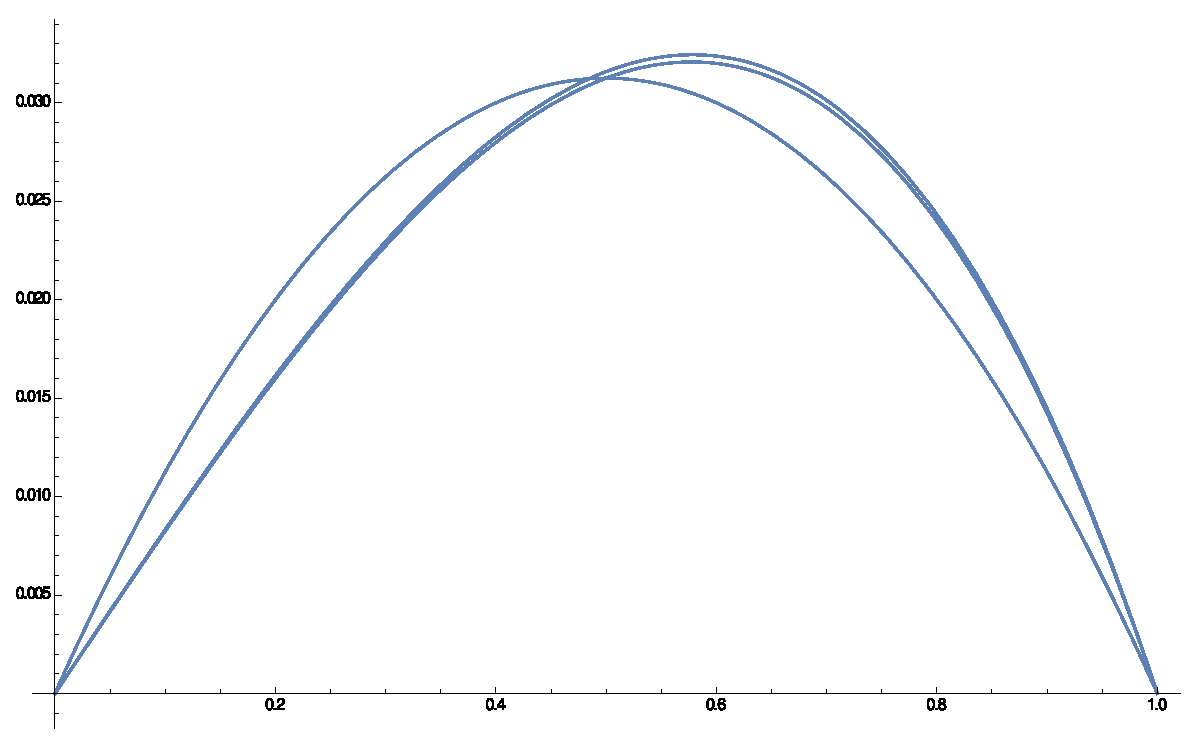
\includegraphics[width=0.5\columnwidth]{optics.eps}
\end{figure}



\subsection*{Задача 2 (статика и теория упругости)}

Пусть имеется цепочка из $N$ точечных масс $\tilde{m}$, соединённых
пружинками жёсткостью $\tilde{k}$; пружинки в нерастянутом состоянии
имеют длину $a$. Первый шарик закрепляют в точке $(0;0)$, а последний
- в точке $(L;0)$ (ось $y$ направлена вертикально вверх). Под действием
силы тяжести, цепочка провисает. Исследуем это провисание в пределе
$N\to\infty$.\\\\
Чтобы задача имела конечный предел $N\to\infty$, параметры задачи
тоже нужно менять в зависимости от $N$. Эта задача является моделью
упругого тела (пружины) массы $M$ и жёсткостью $k$, которая провисает
под собственным весом. Если это так, то жёсткости каждой из маленьких
пружинок выражаются как $\tilde{k}=k\frac{L}{a}=kN$, а массы равны
$\tilde{m}=M\frac{a}{L}=\frac{M}{N}$.


\subsubsection*{Решение}

Пусть координаты каждого из шариков $\{(x_{n},y_{n})\}_{n=1}^{N}$.
Потенциальная энергия складывается из двух вкладов: во-первых, это
потенциальная энергия в поле тяжести, а во-вторых, энергия растяжения
пружинок:

\[
U_{1}=\sum_{n=1}^{N}\tilde{m}gy_{n}
\]


\[
U_{2}=\sum_{n=1}^{N-1}\frac{1}{2}\tilde{k}\left[\sqrt{\left(x_{n+1}-x_{n}\right)^{2}+\left(y_{n+1}-y_{n}\right)^{2}}-a\right]^{2}
\]

\noindent
Проведём теперь переход к пределу $N\to\infty$. Для этого введём
вместо $x_{n}$ и $y_{n}$ непрерывные функции $x(l=na)\equiv x_{n}$
и $y(l=na)\equiv y_{n}$ и $l\in[0,L]$. Во-вторых, заменим суммы
на интегралы по правилу $\sum_{n=1}^{N}\mapsto\int_{0}^{L}\frac{dl}{a}$.
Наконец, конечные разности, стоящие под корнем, выразим через производные.
Получим следующий функционал энергии:

\[
U[x(l),y(l)]=\int_{0}^{L}dl\left[\frac{1}{2}kL\left(\sqrt{x^{\prime2}+y^{\prime2}}-1\right)^{2}+\frac{1}{L}Mgy\right]
\]

\noindent
Во-первых, мы избавились от всех бесконечно малых и бесконечно больших
величин, оставшиеся величины имеют конечный предел при $N\to\infty$.
Это явный признак того, что мы правильно выбрали зависимость параметров
исходной задачи от $N$ для воспроизведения непрерывного предела.
Во-вторых, физический смысл $x(l)$ и $y(l)$ можно понять следующим
образом. Пусть в какой-то момент гравитацию ``выключили''; при этом
пружинка будет располагаться в горизонтальном положении; и $x(l)=l$
и $y(l)=0$. После ``включения'' гравитации, пружина провиснет,
при этом точка, которая изначально имела координаты $(l,0)$ переместится
в точку $(x(l),y(l))$. Наконец, обезразмерим задачу, введя следующие
параметры: $\tilde{x}=\frac{x}{L}$, $\tilde{y}=\frac{y}{L}$, $\tilde{l}=\frac{l}{L}$,$\varkappa=\frac{Mg}{kL}$,
$\tilde{U}=\frac{U}{kL^{2}}$. Получим:

\[
U\left[x(l),y(l)\right]=\int_{0}^{1}dl\left[\frac{1}{2}\left(\sqrt{x^{\prime}(l)^{2}+y^{\prime}(l)^{2}}-1\right)^{2}+\varkappa y(l)\right],
\quad x(0)=y(0)=y(1)=0,x(1)=1
\]

\noindent
Тут и далее, как всегда, все знаки ``\textasciitilde{}'' будут опускаться.
Поскольку мы предполагаем провис маленьким (иначе теория упругости,
вообще говоря, не работает) - это значит, что параметр $\kappa\ll1$.


\paragraph{Размерный анализ}

Получим из соображений размерности характерную высоту провисания пружинки.
Пусть пружинка провисла на величину $h$. Тогда в интеграле можно
сделать следующие оценки: $x^{\prime}\sim1$, $y\sim-h$, $y^{\prime}\sim-h$
(напомним, что в обезразмеренной задаче $L=1$; иначе оцена выглядела
бы как $y^{\prime}\sim-\frac{h}{L}$). Таким образом, потенциальная
энергия имеет вид:
\[
U\sim h^{4}-\kappa h
\]

\noindent
Имеется противоборство двух вкладов: член $\sim\kappa h$, связанный
с силой тяжести, стремится к наибольшему провисанию, в то время как
член $\sim h^{4}$, связанный с упругой энергией, стремится ``выровнять''
пружинку и минимизировать провисание. Равновесие наступает, когда
эти вклады примерно одинаковы, что дает нам размерную оценку на масштаб
величины провисания:
\[
h^{4}\sim\kappa h\Rightarrow h\sim\kappa^{1/3}
\]

\noindent
Потенциальная энергия при этом имеет масштаб:
\[
U\sim h^{4}\sim\kappa^{4/3}
\]

\noindent
(напомним, что мы рабоаем в обезразмеренных единицах; в исходной задаче
$h\sim L\kappa^{1/3}$). 


\paragraph{Пробная функция}

В качестве пробной функции мы будем рассматривать параболы. Однако
заметим, что параметризация $x(l)$ и $y(l)$ уже фиксирована; поэтому
сделаем дополнительное приближение, а именно, мы пренебрежем смещением
элементов пружины по горизонтали. Это приближение соответствует подстановке
следующих пробных функций: 
\[
\begin{cases}
x(l) & =l\\
y(l) & =-\alpha l(1-l)
\end{cases}
\]

\noindent
(знак перед $\alpha>0$ выбран так, чтобы явно отразить тот факт,
что пружинка будет провисать вниз). Подставляя её в приближенный функционал:
\[
U[x(l),y(l)]=\int_{0}^{1}dl\left[\frac{1}{2}\left(\sqrt{1+y^{\prime}(l)^{2}}-1\right)^{2}+\varkappa y(l)\right]
\approx\int_{0}^{1}dl\left[\frac{1}{8}y^{\prime4}+\varkappa y\right]=\frac{\alpha^{4}}{40}-\frac{\alpha\kappa}{6}
\]

\noindent
Минимум достигается при $\alpha=\left(\frac{5}{3}\kappa\right)^{1/3}$;
при этом энергия равна $U=-\frac{1}{8}\left(\frac{5}{3}\right)^{1/3}\kappa{}^{4/3}\approx-0.148\cdot kL^{2}\left(\frac{Mg}{kL}\right)^{4/3}$;
максимальное провисание равно $h=-y(\frac{1}{2})=\frac{1}{4}\left(\frac{5}{3}\kappa\right)^{1/3}\approx0.296\kappa^{1/3}$.


\paragraph{Аналитическое приближенное решение}

Сделаем то же приближение $x(l)=l$; но при этом не будем ничего предполагать
про $y(l)$, кроме её малости. В таком случае энергия запишется как:

\[
U[x(l),y(l)]\approx\int_{0}^{1}dl\left[\frac{1}{8}y^{\prime4}+\varkappa y\right]
\]

\noindent
Уравнение Эйлера-Лагранжа для этой задачи и его решение записывается
следующим образом:

\[
\frac{d}{dl}\left(\frac{1}{2}y^{\prime3}\right)=\kappa\Rightarrow y^{\prime}(l)=\sqrt[3]{2\kappa(l-l_{0})}
\Rightarrow
y(l)=(2\kappa)^{1/3}\cdot\frac{3}{4}(l-l_{0})^{4/3}+y_{0}=\frac{3}{8}\kappa^{1/3}\left((2l-1)^{4/3}-1\right)
\]

\noindent
Можно сравнить это решение с предыдущим. Энергия равна $U=-\frac{9}{56}\kappa^{4/3}\approx-0.161\kappa^{4/3}$
(то есть это приближение лучше предыдущего); максимальное провисание
равно $h=-y(\frac{1}{2})=\frac{3}{8}\kappa^{1/3}=0.375\kappa^{1/3}$.


\paragraph{Численное решение}

Точные уравнения Эйлера-Лагранжа записываются как:
\[
x^{\prime}y^{\prime}y^{\prime\prime}+x^{\prime2}x^{\prime\prime}\sqrt{x^{\prime2}+y^{\prime2}}+x^{\prime\prime}y^{\prime2}\left(\sqrt{x^{\prime2}+y^{\prime2}}-1\right) =0
\]
\[
x^{\prime2}\left(\kappa\sqrt{x^{\prime2}+y^{\prime2}}-2y^{\prime\prime}\left(\sqrt{x^{\prime2}+y^{\prime2}}-1\right)\right)+\\
+y^{\prime2}\sqrt{x^{\prime2}+y^{\prime2}}(\kappa-2y^{\prime\prime})-2x^{\prime}x^{\prime\prime}y^{\prime} =0
\]

\noindent
Это уравнение можно решать численно, сравнивая с аналитичесими приближениями.

\begin{figure}[h]
\caption{Приближение к решению и точное решение при $\kappa=0.5$}
\centering
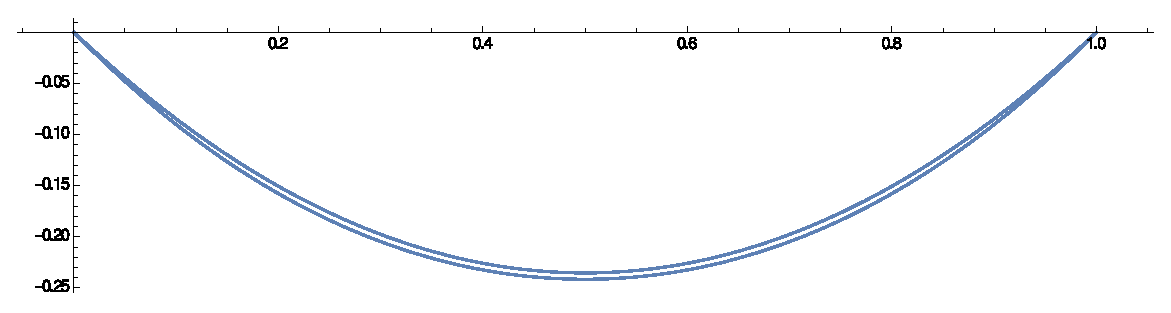
\includegraphics[width=0.8\columnwidth]{static.eps}
\end{figure}


\subsection*{Задачи для домашнего решения}

\noindent \textbf{Упражнение 1}

\noindent Используя кубическую пробную функцию, получить наилучшее приближенное решение для движения луча в среде с $n(x,y)=n_0 - \beta x y$ между двумя точками $x=0$, $y=0$ и $x=L$, $y=0$. Считать, что $\beta L^2\ll n_0$.

\vspace{15pt}
\noindent \textbf{Упражнение 2}

\noindent Рассмотрите задачу про провисание пружины в случае, когда в нерастянутом состоянии длина пружины $L_0$ много меньше расстояния между точками закрепления $L$. Параметр $\kappa = Mg/kL$ считать малым: $\kappa\ll 1$.

\vspace{15pt}
\noindent \textbf{Упражнение 3}

\noindent Показатель преломления в атмосфере меняется с высотой как $n(z)=n_0(1-\alpha z)$. Исследуйте, под каким углом будет видно точечный источник находящийся на расстоянии $d$ от наблюдателя, таком что $\alpha d\ll 1$

\vspace{15pt}
\noindent \textbf{Задача 1}

\noindent Между двумя кольцами радиуса $R$, разведенными на расстояние $d$, натянута мыльная пленка. Энергия пленки пропорциональна ее площади. Определите точно профиль пленки и найдите ее прогиб при $d\ll R$.
\end{document}
